\documentclass[a4paper,12pt]{article}

\usepackage{float}


\usepackage[utf8]{inputenc}
\usepackage[dvips]{graphicx}
%\usepackage{a4wide}
\usepackage{epsfig}
\usepackage{fancybox}
\usepackage{verbatim}
\usepackage{array}
\usepackage{latexsym}
\usepackage{alltt}
\usepackage{amssymb}
\usepackage{amsmath,amsthm}
\usepackage{bm}
\usepackage{wasysym}

%\usepackage{fullpage}
%\usepackage{hyperref}
\usepackage{listings}
\usepackage{color}
\usepackage{algorithm}
\usepackage{algpseudocode}
\usepackage[hmargin=2cm,vmargin=3.0cm]{geometry}
%\topmargin=0cm
%\topmargin=-1.8cm
%\addtolength{\textheight}{6.5cm}
%\addtolength{\textwidth}{2.0cm}
%\setlength{\leftmargin}{-3cm}
%\setlength{\oddsidemargin}{0.0cm}
%\setlength{\evensidemargin}{0.0cm}

%misc libraries goes here
\usepackage{tikz}
\usepackage{tikz-qtree}
\usetikzlibrary{automata,positioning}

\usepackage{multicol}
\usepackage{enumitem}

\usepackage[most]{tcolorbox}

\usepackage[colorlinks=true,urlcolor=black,linkcolor=black]{hyperref}


\lstdefinestyle{customtex}{
    %backgroundcolor=\color{lbcolor},
    tabsize=2,
    language=TeX,
    numbers=none,
    basicstyle=\footnotesize\ttfamily,
    numberstyle=\footnotesize,
    aboveskip={0.0\baselineskip},
    belowskip={0.0\baselineskip},
    %
    columns=flexible,
    keepspaces=true,
    fontadjust=true,
    upquote=true,
    %
    breaklines=true,
    prebreak=\raisebox{0ex}[0ex][0ex]{\ensuremath{\hookleftarrow}},
    frame=single,
    showtabs=false,
    showspaces=false,
    showstringspaces=false,
    %
    %identifierstyle=\color[rgb]{0,0.2,0.8},
    identifierstyle=\color[rgb]{0,0,0.5},
    %identifierstyle=\color[rgb]{0.133,0.545,0.133},
    %keywordstyle=\color[rgb]{0.8,0,0},
    %keywordstyle=\color[rgb]{0.133,0.545,0.133},
    keywordstyle=\color[rgb]{0,0,0.5},
    %commentstyle=\color[rgb]{0.133,0.545,0.133},
    commentstyle=\color[rgb]{0.545,0.545,0.545},
    %stringstyle=\color[rgb]{0.827,0.627,0.133},
    stringstyle=\color[rgb]{0.133,0.545,0.133},
    %
    literate={â}{{\^{a}}}1 {Â}{{\^{A}}}1 {ç}{{\c{c}}}1 {Ç}{{\c{C}}}1 {ğ}{{\u{g}}}1 {Ğ}{{\u{G}}}1 {ı}{{\i}}1 {İ}{{\.{I}}}1   {ö}{{\"o}}1 {Ö}{{\"O}}1 {ş}{{\c{s}}}1 {Ş}{{\c{S}}}1 {ü}{{\"u}}1 {Ü}{{\"U}}1 {~}{$\sim$}{1}
}

\lstdefinestyle{output}{
    %backgroundcolor=\color{lbcolor},
    tabsize=2,
    numbers=none,
    basicstyle=\footnotesize\ttfamily,
    numberstyle=\footnotesize,
    aboveskip={0.0\baselineskip},
    belowskip={0.0\baselineskip},
    %
    columns=flexible,
    keepspaces=true,
    fontadjust=true,
    upquote=true,
    %
    breaklines=true,
    prebreak=\raisebox{0ex}[0ex][0ex]{\ensuremath{\hookleftarrow}},
    frame=single,
    showtabs=false,
    showspaces=false,
    showstringspaces=false,
    %
    %identifierstyle=\color[rgb]{0.44,0.12,0.1},
    identifierstyle=\color[rgb]{0,0,0},
    keywordstyle=\color[rgb]{0,0,0},
    commentstyle=\color[rgb]{0,0,0},
    stringstyle=\color[rgb]{0,0,0},
    %
    literate={â}{{\^{a}}}1 {Â}{{\^{A}}}1 {ç}{{\c{c}}}1 {Ç}{{\c{C}}}1 {ğ}{{\u{g}}}1 {Ğ}{{\u{G}}}1 {ı}{{\i}}1 {İ}{{\.{I}}}1   {ö}{{\"o}}1 {Ö}{{\"O}}1 {ş}{{\c{s}}}1 {Ş}{{\c{S}}}1 {ü}{{\"u}}1 {Ü}{{\"U}}1
}

\lstset{style=customtex}


\tikzset{%
    terminal/.style={draw, rectangle,
    				 align=center, 
					 minimum height=1cm, 
					 minimum width=2cm,
					 fill=black!10,
					 anchor=mid},
    nonterminal/.style={draw, rectangle,
    					align=left,
					    minimum height=1cm, 
						minimum width=2cm, 
						anchor=mid},% and so on
}

%% Style for terminals
%\tikzstyle{terminal}=[draw, rectangle, 
%					  minimum height=1cm, 
%					  minimum width=2cm, 
%					  fill=black!20,
%					  anchor=south west]
%% Style for nonterminals
%\tikzstyle{nonterminal}=[draw, rectangle, 
%						 minimum height=1 cm, 
%						 minimum width=2 cm, 
%						 anchor=north east]


\newcommand{\HRule}{\rule{\linewidth}{1mm}}
\newcommand{\kutu}[2]{\framebox[#1mm]{\rule[-2mm]{0mm}{#2mm}}}
\newcommand{\gap}{ \\[1mm] }

\newcommand{\Q}{\raisebox{1.7pt}{$\scriptstyle\bigcirc$}}
\newcommand{\minus}{\scalebox{0.35}[1.0]{$-$}}

\setlength{\fboxsep}{10pt}

\tcbsetforeverylayer{enhanced jigsaw, breakable, arc=0mm, boxrule=1pt, boxsep=5pt, after=\vspace{1em}, colback=white, colframe=black}

\newcolumntype{P}[1]{>{\centering\arraybackslash}p{#1}}

\setlength\parindent{0pt}

%\renewcommand\arraystretch{1.2}

\newenvironment{Tab}[1]
  {\def\arraystretch{1}\tabular{#1}}
  {\endtabular}

%%%%%%%%%%%%%%%%%%%%%%%%%%%%%%%%%%%%%%%%%%%%%%%%%%%%%%%%%%%%%%%%%%%%%%%%%%%%%%%%%%%%%%

\title{Formal Languages and Abstract Machines \\ Take Home Exam 2}
\author{Mert AKÇA \\ 2171163 } % write your name and id
\date{} % do not write any date

%%%%%%%%%%%%%%%%%%%%%%%%%%%%%%%%%%%%%%%%%%%%%%%%%%%%%%%%%%%%%%%%%%%%%%%%%%%%%%%%%%%%%%

\begin{document}
\HRule\\
Middle East Technical University \hfill Department of Computer Engineering
{\let\newpage\relax\maketitle}
\HRule\\
\vspace{1cm}

%%%%%%%%%%%%%%%%%%%%%%%%%%%%%%%%%%%%%%%%%%%%%%%%%%%%%%%%%%%%%%%%%%%%%%%%%%%%%%%%%%%%%%

% Write your answers below the section tags
\section{Context-Free Grammars \hfill \normalfont{(10 pts)}}

\paragraph{a)} Give the rules of the Context-Free Grammars to recognize strings in the given languages where $\Sigma=\{a,b\}$ and $S$ is the start symbol. \\  

$L(G)=\{w \mid \;  w \in \Sigma^*;\; |w| \geq 3;\; $  \hfill \small{(2/10 pts)} \\
\hspace*{22mm} the first and the second from the last symbols of $w$ are the same$\}$ \\

\begin{tcolorbox}
$S \to Aaa$, \\
$S \to Abb$, \\
$A \to Ba$, \\
$A \to Bb$, \\
$B \to Bb\ |\ Ba\ |\ e$ \\
\end{tcolorbox}


$L(G)=\{w \mid \;  w \in \Sigma^*;\; $ the length of w is odd$\}$ \hfill \small{(2/10 pts)} \\

\begin{tcolorbox}
$S \to AaA\ |\ AbA$ \\
$A \to aAa \ |\ aAb \ |\ bAa \ | \ bAb \ |\ e$ \\
\end{tcolorbox}


$L(G)=\{w \mid \;  w \in \Sigma^*;\; n(w,a)=2\cdot n(w,b)\}$ where $n(w,x)$ is the number of $x$ symbols in $w$ \hfill \small{(3/10 pts)} \\

\begin{tcolorbox}
$S \to A\ |\ e$ \\
$A \to aAaAb\ |\ aAbAa\ |\ bAaAa\ |\ e$ \\
\end{tcolorbox}



\paragraph{b)} Find the set of strings recognized by the CFG rules given below:         \hfill \small{(3/10 pts)} \\


$S \to X \mid Y$ \\
$X \to aXb \mid A \mid B$ \\
$A \to aA \mid a$ \\
$B \to Bb \mid b$ \\
$Y \to CbaC$ \\
$C \to CC \mid a \mid b \mid \varepsilon$  \\

\begin{tcolorbox}
L(G) = $\{a^n(a^+\cup b^+)b^n, (a\cup b)^*ba(a\cup b)^* \}$
\end{tcolorbox}


\newpage
\section{Parse Trees and Derivations \hfill \normalfont{(20 pts)}}
Given the CFG below, provide parse trees for given sentences in \textbf{a} and \textbf{b}.\\

\begin{lstlisting}[style=output,mathescape=true]
S   $\to$ NP VP
VP  $\to$ V NP | V NP PP
PP  $\to$ P NP
NP  $\to$ N | D N | NP PP
V   $\to$ wrote | built | constructed
D   $\to$ a | an | the | my
N   $\to$ John | Mary | Jane | man | book | automata | pen | class
P   $\to$ in | on | by | with
\end{lstlisting}

\paragraph{a)} Jane constructed automata with a pen \hfill \small{(4/20 pts)} \\

\begin{tcolorbox}
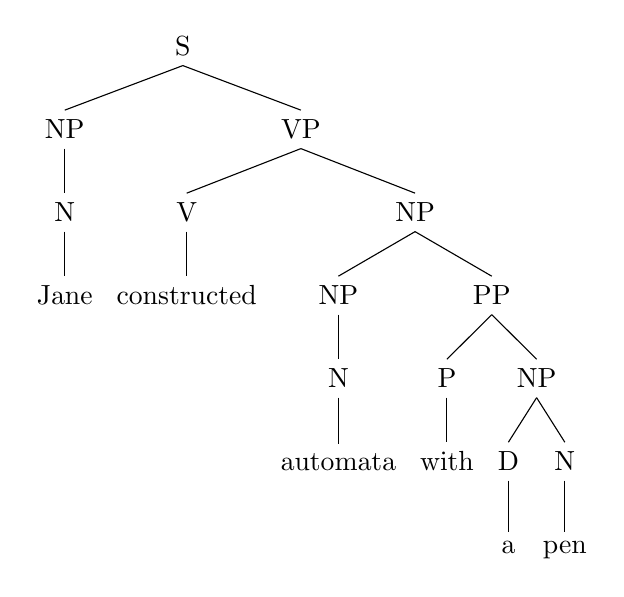
\begin{tikzpicture}[scale=1]
\Tree [.S [.\node(site){NP}; [.N Jane ] ] 
          [.VP [.V constructed ] 
               [.NP [.\node(site){NP}; [.N automata ] ] 
                    [.PP [.P with ] [.NP [.D a ] [.N pen ] ] ] ] ] ]
\end{tikzpicture}
\end{tcolorbox}

\paragraph{b)} my book in the man built a Jane by a pen \hfill \small{(4/20 pts)} \\

\begin{tcolorbox}
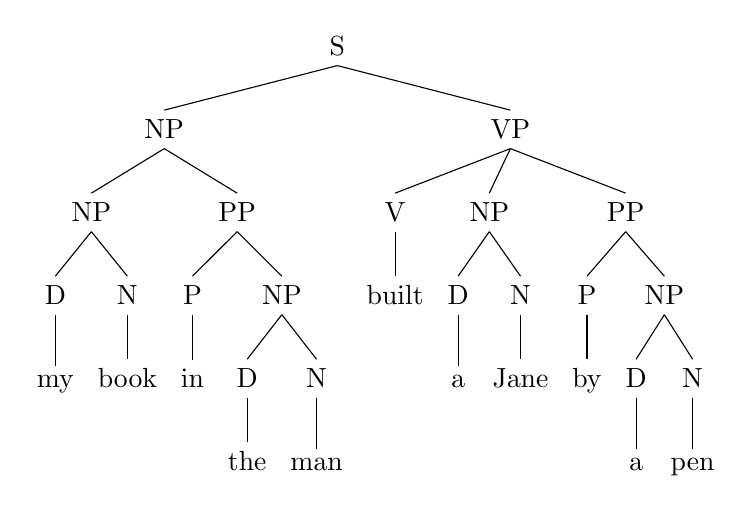
\begin{tikzpicture}[scale=1]
\Tree [.S [.NP [.NP [.D my ][.N book ] ] [.PP [.P in ] [.NP [.D the ] [.N man ] ] ] ] 
          [.VP [.V built ] 
               [.NP [.D a ] [.N Jane ] ] 
               [.PP [.P by ] [.NP [.D a ] [.N pen ] ] ] ] ]
\end{tikzpicture}
\end{tcolorbox}

\newpage

Given the CFG below, answer \textbf{c}, \textbf{d} and \textbf{e} \\

\begin{lstlisting}[style=output,mathescape=true]
S  $\to$ E
E  $\to$ E + T | E - T | T
T  $\to$ T * I | T / I | I
I  $\to$ 0 | 1 | 2 | 3 | 4 | 6 | 7 | 8 | 9
\end{lstlisting}

\paragraph{c)} Provide the left-most derivation of 7 - 4 * 3 step-by-step and plot the final parse \hfill \small{(4/20 pts)} \\
tree matching that derivation \\

\begin{tcolorbox}
$D = S \to E \to E - T \to T-T \to I-T \to 7-T \to 7-T*I \to 7-I*I \to 7-4*I \to 7-4*3$ \\

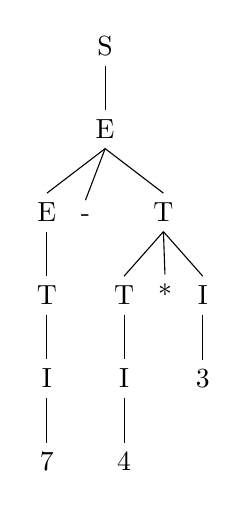
\begin{tikzpicture}[scale=1]
\Tree [.\node(site){S}; [.E [.\node(site){E}; [.\node(site){T}; [.I 7 ] ] ]
                            [.- ]
                            [.T [.\node(site){T}; [.I 4 ]  ] [.* ] [.I 3 ] ]
                              ] ]
\end{tikzpicture}
\end{tcolorbox}

\paragraph{d)} Provide the right-most derivation of 7 - 4 * 3 step-by-step and plot the final parse \hfill \small{(4/20 pts)} \\
 tree matching that derivation \\
 
\begin{tcolorbox}
$D = S \to E \to E-T \to E-T*I \to E-T*3 \to E - I*3 \to E - 4*3 \to T-4*3 \to I - 4*3 \to 7-4*3$ \\ 

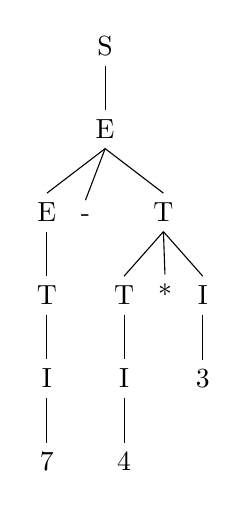
\begin{tikzpicture}[scale=1]
\Tree [.\node(site){S}; [.E [.\node(site){E}; [.\node(site){T}; [.I 7 ] ] ]
                            [.- ]
                            [.T [.\node(site){T}; [.I 4 ]  ] [.* ] [.I 3 ] ]
                              ] ]
\end{tikzpicture}
\end{tcolorbox}


\paragraph{e)} Are the derivations in \textbf{c} and \textbf{d} in the same similarity class?  \hfill \small{(4/20 pts)} \\

\begin{tcolorbox}
Yes, their final parse trees are the same
\end{tcolorbox}


\newpage
\section{Pushdown Automata \hfill \normalfont{(30 pts)}}

\paragraph{a)} 
Find the language recognized by the PDA given below \hfill \small{(5/30 pts)} \\

\begin{tikzpicture}[shorten >=1pt,node distance=3cm,on grid,auto]
\node[state,initial,initial text=] (q_0) {$q_0$};
\node[state] (q_1) [right=of q_0] {$q_1$};
\node[state] (q_2) [above right=of q_1] {$q_2$};
\node[state] (q_3) [below right=of q_1] {$q_3$};
\node[state,accepting](q_4) [right=of q_2] {$q_4$};
\node[state](q_5) [right=of q_3] {$q_5$};
\node[state,accepting](q_6) [right=of q_5] {$q_6$};
\path[->]

(q_0) edge node {$\varepsilon,\varepsilon \to \#$} (q_1)
(q_1) edge [loop below] node {$x,\varepsilon \to x$} (q_1)

%%
(q_1) edge node {$\varepsilon,\varepsilon \to \varepsilon$} (q_2)
(q_2) edge [loop above] node {$y,x \to \varepsilon$} (q_2)

(q_2) edge node {$\varepsilon,\# \to \varepsilon$} (q_4)
(q_4) edge [loop above] node {$z,\varepsilon \to \varepsilon$} (q_4)

%%%

(q_1) edge node {$\varepsilon,\varepsilon \to \varepsilon$} (q_3)
(q_3) edge [loop below] node {$y,\varepsilon \to \varepsilon$} (q_3)

(q_3) edge node {$\varepsilon,\varepsilon \to \varepsilon$} (q_5)
(q_5) edge [loop below] node {$z,x \to \varepsilon$} (q_5)

(q_5) edge node {$\varepsilon,\# \to \varepsilon$} (q_6)
;
\end{tikzpicture} \\

\begin{minipage}{0.60\textwidth}
where the transition $((q_i,\alpha,\beta),(q_j,\gamma)) $ is represented as: 
\end{minipage}
\begin{minipage}{0.30\textwidth}
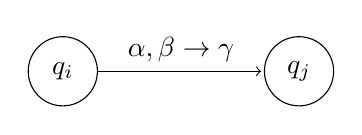
\begin{tikzpicture}[shorten >=1pt,node distance=3cm,on grid,auto]
\node[state] (q_i) {$q_i$};
\node[state] (q_j) [right=of q_i] {$q_j$};
\path[->]
(q_i) edge node {$\alpha,\beta \to \gamma$} (q_j);
\end{tikzpicture} \\
\end{minipage}


\begin{tcolorbox}
L = $x^ny^nz^*$ or $x^ny^*z^n$, where $n \in N$
\end{tcolorbox}


\paragraph{b)} 
Design a PDA to recognize language $ L=\{x^n y^{m+n} x^m \mid \; n,m \geq 0; \; n,m \in \mathbb{N}  \} $  \hfill \small{(5/30 pts)} \\

\begin{tcolorbox}
$ \to q_0$ is the start state
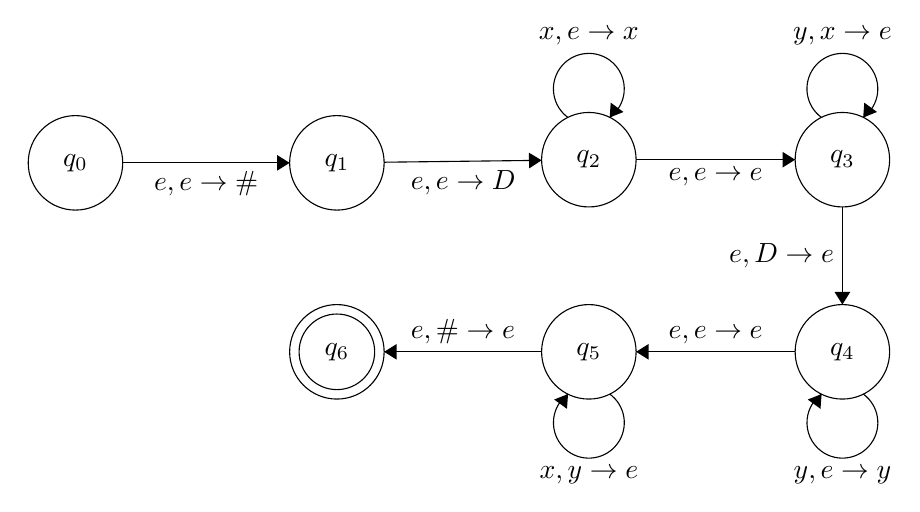
\begin{tikzpicture}[scale=0.2]
\tikzstyle{every node}+=[inner sep=0pt]
\draw [black] (3.5,-20.9) circle (3);
\draw (3.5,-20.9) node {$q_0$};
\draw [black] (20.1,-20.9) circle (3);
\draw (20.1,-20.9) node {$q_1$};
\draw [black] (36.1,-20.7) circle (3);
\draw (36.1,-20.7) node {$q_2$};
\draw [black] (52.2,-20.7) circle (3);
\draw (52.2,-20.7) node {$q_3$};
\draw [black] (52.2,-32.9) circle (3);
\draw (52.2,-32.9) node {$q_4$};
\draw [black] (36.1,-32.9) circle (3);
\draw (36.1,-32.9) node {$q_5$};
\draw [black] (20.1,-32.9) circle (3);
\draw (20.1,-32.9) node {$q_6$};
\draw [black] (20.1,-32.9) circle (2.4);
\draw [black] (6.5,-20.9) -- (17.1,-20.9);
\fill [black] (17.1,-20.9) -- (16.3,-20.4) -- (16.3,-21.4);
\draw (11.8,-21.4) node [below] {$e,e \to \#$};
\draw [black] (23.1,-20.86) -- (33.1,-20.74);
\fill [black] (33.1,-20.74) -- (32.29,-20.25) -- (32.31,-21.25);
\draw (28.12,-21.36) node [below] {$e,e \to D$};
\draw [black] (39.1,-20.7) -- (49.2,-20.7);
\fill [black] (49.2,-20.7) -- (48.4,-20.2) -- (48.4,-21.2);
\draw (44.15,-21.2) node [below] {$e,e \to e$};
\draw [black] (34.777,-18.02) arc (234:-54:2.25);
\draw (36.1,-13.45) node [above] {$x,e \to x$};
\fill [black] (37.42,-18.02) -- (38.3,-17.67) -- (37.49,-17.08);
\draw [black] (50.877,-18.02) arc (234:-54:2.25);
\draw (52.2,-13.45) node [above] {$y, x \to e$};
\fill [black] (53.52,-18.02) -- (54.4,-17.67) -- (53.59,-17.08);
\draw [black] (52.2,-23.7) -- (52.2,-29.9);
\fill [black] (52.2,-29.9) -- (52.7,-29.1) -- (51.7,-29.1);
\draw (51.7,-26.8) node [left] {$e, D \to e$};
\draw [black] (49.2,-32.9) -- (39.1,-32.9);
\fill [black] (39.1,-32.9) -- (39.9,-33.4) -- (39.9,-32.4);
\draw (44.15,-32.4) node [above] {$e, e \to e$};
\draw [black] (53.523,-35.58) arc (54:-234:2.25);
\draw (52.2,-40.15) node [below] {$y,e \to y$};
\fill [black] (50.88,-35.58) -- (50,-35.93) -- (50.81,-36.52);
\draw [black] (37.423,-35.58) arc (54:-234:2.25);
\draw (36.1,-40.15) node [below] {$x,y \to e$};
\fill [black] (34.78,-35.58) -- (33.9,-35.93) -- (34.71,-36.52);
\draw [black] (33.1,-32.9) -- (23.1,-32.9);
\fill [black] (23.1,-32.9) -- (23.9,-33.4) -- (23.9,-32.4);
\draw (28.1,-32.4) node [above] {$e,\# \to e$};
\end{tikzpicture}
\end{tcolorbox}

\newpage

\paragraph{c)} 
Design a PDA to recognize language $ L=\{x^n y^m \mid \; n < m \leq 2n; \; n,m \in \mathbb{N^+} \} $  \hfill \small{(10/30 pts)} \\
Do not use multi-symbol push/pop operations in your transitions. \\
Simulate the PDA on strings \textit{xxy} (with only one rejecting derivation) and \textit{xxyyyy} (accepting derivation) with transition tables. \\


\begin{tcolorbox}

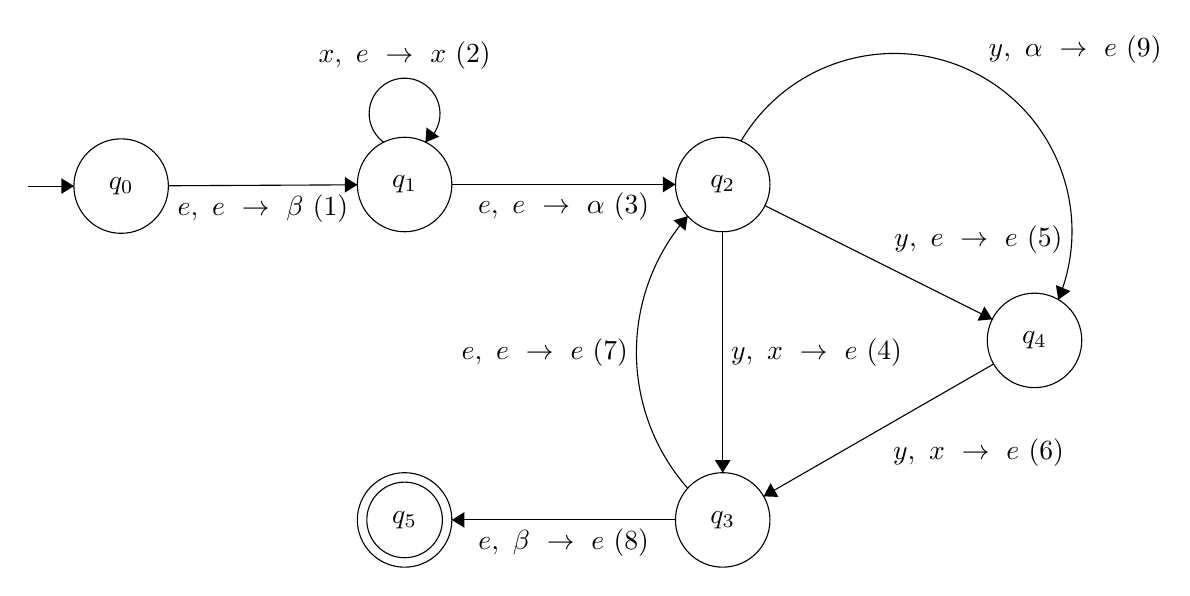
\begin{tikzpicture}[scale=0.2]
\tikzstyle{every node}+=[inner sep=0pt]
\draw [black] (10.9,-12.8) circle (3);
\draw (10.9,-12.8) node {$q_0$};
\draw [black] (28.9,-12.7) circle (3);
\draw (28.9,-12.7) node {$q_1$};
\draw [black] (49.1,-12.7) circle (3);
\draw (49.1,-12.7) node {$q_2$};
\draw [black] (49.1,-34) circle (3);
\draw (49.1,-34) node {$q_3$};
\draw [black] (68.9,-22.6) circle (3);
\draw (68.9,-22.6) node {$q_4$};
\draw [black] (28.9,-34) circle (3);
\draw (28.9,-34) node {$q_5$};
\draw [black] (28.9,-34) circle (2.4);
\draw [black] (5,-12.8) -- (7.9,-12.8);
\fill [black] (7.9,-12.8) -- (7.1,-12.3) -- (7.1,-13.3);
\draw [black] (13.9,-12.78) -- (25.9,-12.72);
\fill [black] (25.9,-12.72) -- (25.1,-12.22) -- (25.1,-13.22);
\draw (19.9,-13.29) node [below] {$e,\mbox{ }e\mbox{ }\to\mbox{ }\beta\mbox{ }(1)$};
\draw [black] (31.9,-12.7) -- (46.1,-12.7);
\fill [black] (46.1,-12.7) -- (45.3,-12.2) -- (45.3,-13.2);
\draw (39,-13.2) node [below] {$e,\mbox{ }e\mbox{ }\to\mbox{ }\alpha\mbox{ }(3)$};
\draw [black] (27.577,-10.02) arc (234:-54:2.25);
\draw (28.9,-5.45) node [above] {$x,\mbox{ }e\mbox{ }\to\mbox{ }x\mbox{ }(2)$};
\fill [black] (30.22,-10.02) -- (31.1,-9.67) -- (30.29,-9.08);
\draw [black] (51.78,-14.04) -- (66.22,-21.26);
\fill [black] (66.22,-21.26) -- (65.72,-20.45) -- (65.28,-21.35);
\draw (65.34,-17.12) node [above] {$y,\mbox{ }e\mbox{ }\to\mbox{ }e\mbox{ }(5)$};
\draw [black] (66.3,-24.1) -- (51.7,-32.5);
\fill [black] (51.7,-32.5) -- (52.64,-32.54) -- (52.14,-31.67);
\draw (65.34,-28.81) node [below] {$y,\mbox{ }x\mbox{ }\to\mbox{ }e\mbox{ }(6)$};
\draw [black] (49.1,-15.7) -- (49.1,-31);
\fill [black] (49.1,-31) -- (49.6,-30.2) -- (48.6,-30.2);
\draw (49.6,-23.35) node [right] {$y,\mbox{ }x\mbox{ }\to\mbox{ }e\mbox{ }(4)$};
\draw [black] (46.879,-31.993) arc (-138.67184:-221.32816:13.088);
\fill [black] (46.88,-14.71) -- (45.98,-14.98) -- (46.73,-15.64);
\draw (43.12,-23.35) node [left] {$e,\mbox{ }e\mbox{ }\to\mbox{ }e\mbox{ }(7)$};
\draw [black] (46.1,-34) -- (31.9,-34);
\fill [black] (31.9,-34) -- (32.7,-34.5) -- (32.7,-33.5);
\draw (39,-34.5) node [below] {$e,\mbox{ }\beta\mbox{ }\to\mbox{ }e\mbox{ }(8)$};
\draw [black] (50.262,-9.944) arc (149.53727:-22.66737:11.288);
\fill [black] (70.41,-20.02) -- (71.18,-19.47) -- (70.26,-19.09);
\draw (71.48,-5.04) node [above] {$y,\mbox{ }\alpha\mbox{ }\to\mbox{ }e\mbox{ }(9)$};
\end{tikzpicture}

\begin{table}[H]
\centering
\caption{Transition Table for xxy}
\label{my-label}
\begin{tabular}{llll}
State & Unread Input & Stack & Transition  \\
$q_0$ & xxy & $e$ & -  \\
$q_1$ & xxy & $\beta$ & 1   \\
$q_1$ & xy & $x\beta$ & 2   \\
$q_1$ & y & $xx\beta$ & 2   \\
$q_2$ & y & $\alpha xx\beta$ & 3  \\
$q_3$ & e & $xx\beta$ & 9  
\end{tabular}
\end{table}

$\beta\ is\ not\ top\ of\ the\ stack\ so\ we\ cannot\ move\ final\ state$

\begin{table}[H]
\centering
\caption{Transition table for xxyyyy}
\label{my-label}
\begin{tabular}{llll}
State & Unread Input & Stack & Transition  \\
$q_0$ & xxyyyy & $e$ & -   \\
$q_1$ & xxyyyy & $\beta$ & 1   \\
$q_1$ & xyyyy & $x\beta$ & 2   \\
$q_1$ & yyyy & $xx\beta$ & 2   \\
$q_2$ & yyyy & $\alpha xx\beta$ & 3   \\
$q_4$ & yyy & $xx\beta$ & 9   \\
$q_3$ & yy & $x\beta$ & 6   \\
$q_2$ & yy & $x\beta$ & 7   \\
$q_4$ & y & $x\beta$ & 5   \\
$q_3$ & e & $\beta$ & 6   \\
$q_5$ & e & $e$ & 8  
\end{tabular}
\end{table}

\end{tcolorbox}


\paragraph{d)} Given two languages $L'$ and $L$ as $L'=\{w \mid \; w\in L; \; |w|=4n+2 \; for\; n\in \mathbb{N} \}$
\hfill \small{(10/30 pts)} \\
If $L$ is a CFL, show that $L'$ is also a CFL by constructing an automaton for $L'$ in terms of another automaton that recognizes $L$. \\


\begin{tcolorbox}
    Let $L''$ be a regular language $L''=\{w\ |\ |w| = 4n+2\ for\ n \in N\}$. This language has a deterministic automaton $M_1 = (K_1,\sum, \delta, s_1, F_1)$ \\
    
    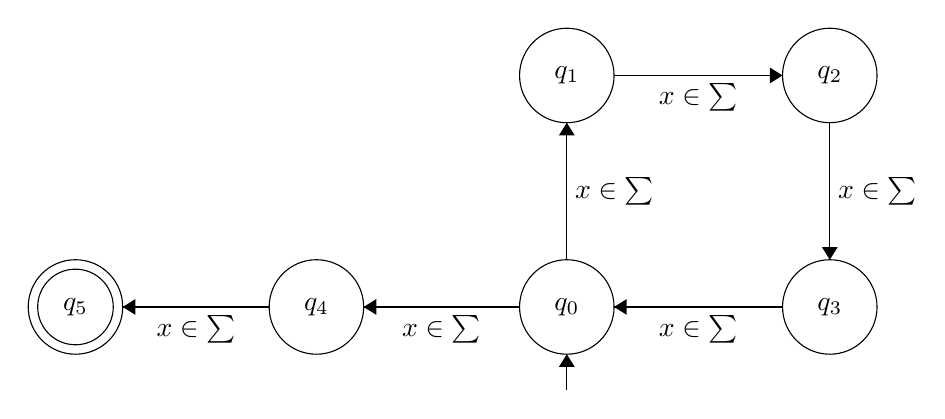
\begin{tikzpicture}[scale=0.2]
\tikzstyle{every node}+=[inner sep=0pt]
\draw [black] (35.5,-24.2) circle (3);
\draw (35.5,-24.2) node {$q_0$};
\draw [black] (35.5,-9.5) circle (3);
\draw (35.5,-9.5) node {$q_1$};
\draw [black] (52.2,-9.5) circle (3);
\draw (52.2,-9.5) node {$q_2$};
\draw [black] (52.2,-24.2) circle (3);
\draw (52.2,-24.2) node {$q_3$};
\draw [black] (19.6,-24.2) circle (3);
\draw (19.6,-24.2) node {$q_4$};
\draw [black] (4.3,-24.2) circle (3);
\draw (4.3,-24.2) node {$q_5$};
\draw [black] (4.3,-24.2) circle (2.4);
\draw [black] (35.5,-29.5) -- (35.5,-27.2);
\fill [black] (35.5,-27.2) -- (35,-28) -- (36,-28);
\draw [black] (35.5,-21.2) -- (35.5,-12.5);
\fill [black] (35.5,-12.5) -- (35,-13.3) -- (36,-13.3);
\draw (36,-16.85) node [right] {$x \in \sum$};
\draw [black] (38.5,-9.5) -- (49.2,-9.5);
\fill [black] (49.2,-9.5) -- (48.4,-9) -- (48.4,-10);
\draw (43.85,-10) node [below] {$x\in \sum$};
\draw [black] (52.2,-12.5) -- (52.2,-21.2);
\fill [black] (52.2,-21.2) -- (52.7,-20.4) -- (51.7,-20.4);
\draw (52.7,-16.85) node [right] {$x \in \sum$};
\draw [black] (49.2,-24.2) -- (38.5,-24.2);
\fill [black] (38.5,-24.2) -- (39.3,-24.7) -- (39.3,-23.7);
\draw (43.85,-24.7) node [below] {$x\in\sum$};
\draw [black] (32.5,-24.2) -- (22.6,-24.2);
\fill [black] (22.6,-24.2) -- (23.4,-24.7) -- (23.4,-23.7);
\draw (27.55,-24.7) node [below] {$x\in\sum$};
\draw [black] (16.6,-24.2) -- (7.3,-24.2);
\fill [black] (7.3,-24.2) -- (8.1,-24.7) -- (8.1,-23.7);
\draw (11.95,-24.7) node [below] {$x\in \sum$};
\end{tikzpicture}

As we can see $L''$ is an regular language because it's accepted by an finite automaton.\\

Intersection of language $L$ and $L''$ (strings with length of 4n+2) is $L'$. L is a CFL and L'' is a regular language, so L' must be also a CFL by Theorem 3.5.2 (textbook, p.144).
\end{tcolorbox}






\newpage
\section{Closure Properties \hfill \normalfont{(20 pts)}}

Let $L_1$ and $L_2$ be context-free languages which are not regular, and let $L_3$ be a regular language. Determine whether the following languages are necessarily CFLs or not. If they need to be context-free, explain your reasoning. If not, give one example where the language is a CFL and a counter example where the language is not a CFL. \\

\paragraph{a)} $L_4 = L_1 \cap (L_2 \setminus L_3)$ \hfill \small{(10/20 pts)} \\

\begin{tcolorbox}
$L_4 = L_1 \cap (L_2 \cap L_3')$ \\
$L_2$ is a CFL and $L_3'$ is a regular language (Complement of a regular language is also regular) so $(L_2 \cap L_3')$ is CFL \\
Therefore, $L_4$ is intersection of two CFL's, so we cannot decide whether it's a CFL or not.
\end{tcolorbox}

\paragraph{b)} $L_5 = (L_1 \cap L_3)\text{*}$ \hfill \small{(10/20 pts)} \\

\begin{tcolorbox}
$(L_1 \cap L_3)$ is intersection of a regular language and context-free lang. so we can say that $(L_1 \cap L_3)$ is CFL \\
Because CFL's are closed under kleene star property $(L_1 \cap L_3)^*$ is also a CFL.
\end{tcolorbox}





\newpage
\section{Pumping Theorem \hfill \normalfont{(20 pts)}}

\paragraph{a)} Show that $L=\{a^n m^n t^i \mid \; n\leq i \leq 2n\}$ is not a Context Free Language \hfill \small{(10/20 pts)} \\
using Pumping Theorem for CFLs. \\

\begin{tcolorbox}
Let pumping length = 4, $|vxy| \le 4 $\\
S = aaaammmmtttt(tttt)\\

Case 1: $|vxy|$ is in the first boundary\\
$aa\underbrace{\hbox{aamm}}_{\hbox{vxy}}mmtttt(tttt)$ for $i=2$; \\
aaaaaammmmmtttt(tttt) : number of a's is not equal to number of m's.\\

Case 2: $|vxy|$ is not in boundary it's in a's or m's \\
$\underbrace{\hbox{aaaa}}_{\hbox{vxy}}mmmmtttt(tttt)$ for $i=2$; \\
aaaaaammmmtttt(tttt) : number of a's is not equal to number of m's.\\
Also:\\
$aaaa\underbrace{\hbox{mmmm}}_{\hbox{vxy}}tttt(tttt)$ for $i=2$; \\
aaaammmmmmtttt(tttt) : number of a's is not equal to number of m's.\\

Case 3: $|vxy|$ is in t's\\
$aaaammmm\underbrace{\hbox{tttt}}_{\hbox{vxy}}(tttt)$ for $i=4$; \\
aaaammmmtttttttttt(tttt) : the mininmum number of t's is greater than 2n.\\

Therefore, the rule is not met in all cases for every $i \ge 0$, this language is not context-free language. 
\end{tcolorbox}


\paragraph{b)} Show that $L=\{a^n b^{2n} a^n \mid \; n \in \mathbb{N+} \}$ is not a Context Free Language \hfill \small{(10/20 pts)} \\
using Pumping Theorem for CFLs. \\

\begin{tcolorbox}
Let pumping length = 3, $|vxy| \le 3 $\\
S = aaabbbbbbaaa\\

Case 1: $|vxy|$ is in the boundaries\\
$a\underbrace{\hbox{$aab$}}_{\hbox{vxy}}bbbbbaaa$ for $i=2$; \\
aaaabbbbbbbaaa : the number of a's is not equal.\\
Also: \\
$aaabbbb\underbrace{\hbox{$bba$}}_{\hbox{vxy}}aa$ for $i=2$; \\
aaabbbbbbbaaaa : the number of a's is not equal.\\

Case 2: $|vxy|$ is not in the boundaries\\
$aaa\underbrace{\hbox{$bbb$}}_{\hbox{vxy}}bbbaaa$ for $i=2$; \\
aaabbbbbbbbaaa : the number of b's is not double of number of a's.\\
Also: \\
$aaabbbbbb\underbrace{\hbox{$aaa$}}_{\hbox{vxy}}$ for $i=2$; \\
aaabbbbbbaaaaa : the number of a's is not equal.\\

Therefore, the rule is not met in all cases for every $i \ge 0$, this language is not context-free language. 
\end{tcolorbox}





\newpage
\section{CNF and CYK \hfill \normalfont{(not graded)}}

\paragraph{a)} Convert the given context-free grammar to Chomsky Normal Form. \\

$ S   \to XSX \mid xY $ \\
$ X   \to Y \mid S $ \\
$ Y   \to z \mid \varepsilon $ \\

\begin{tcolorbox}
answer here ...
\vspace{18cm} % remove this after your answer
\end{tcolorbox}


\paragraph{b)} Use the grammar below to parse the given sentence using Cocke–Younger–Kasami algorithm. \\
Plot the parse trees. \\

\begin{multicols}{2}
S $\to$ NP VP \\
S $\to$ X1 VP \\
X1 $\to$ Aux NP \\
S $\to$ book $\mid$ include $\mid$ prefer \\
S $\to$ Verb NP \\
S $\to$ X2 PP \\
S $\to$ Verb PP \\
S $\to$ VP PP \\
NP $\to$ I $\mid$ she $\mid$ me $\mid$ Houston \\
NP $\to$ Det Nom \\
Nom $\to$ book $\mid$ flight $\mid$ meal $\mid$ money \\
Nom $\to$ Nom Noun \\
Nom $\to$ Nom PP \\
VP $\to$ book $\mid$ include $\mid$ prefer \\
VP $\to$ Verb NP \\
VP $\to$ X2 PP \\
X2 $\to$ Verb NP \\
VP $\to$ Verb PP \\
VP $\to$ VP PP \\
PP $\to$ Prep NP \\
Det $\to$ that $\mid$ this $\mid$ the $\mid$ a \\
Noun $\to$ book $\mid$ flight $\mid$ meal $\mid$ money \\
Verb $\to$ book $\mid$ include $\mid$ prefer \\
Aux $\to$ does \\
Prep $\to$ from $\mid$ to $\mid$ on $\mid$ near $\mid$ through \\
\end{multicols}

\vspace{5mm}

book the flight through Houston \\

\begin{tcolorbox}

\scriptsize

Empty parse table:\\
\begin{tikzpicture}[node distance=0cm, outer sep = 0pt]

\node[terminal] (l0) {
    \begin{tabular}{@{}P{2.9cm}|@{}P{2.9cm}|@{}P{2.9cm}|@{}P{2.9cm}|@{}P{2.9cm}}
    book & the & flight & through & Houston \\
    \end{tabular}
};

\node[nonterminal] (l1) [above = of l0] {
    \begin{tabular}{@{}P{2.9cm}|@{}P{2.9cm}|@{}P{2.9cm}|@{}P{2.9cm}|@{}P{2.9cm}}
    1:1 & 
    2:2 & 
    3:3 & 
    4:4 & 
    5:5 \\
    \end{tabular}
};

\node[nonterminal] (l2) [above = of l1.north] {
    \begin{tabular}{@{}P{2.9cm}|@{}P{2.9cm}|@{}P{2.9cm}|@{}P{2.9cm}}
    1:2 $\to$ 1:1 2:2 & 
    2:3 $\to$ 2:2 3:3 & 
    3:4 $\to$ 3:3 4:4 & 
    4:5 $\to$ 4:4 5:5 \\
    \end{tabular}
};

\node[nonterminal] (l3) [above = of l2.north] {
    \begin{tabular}{@{}P{2.9cm}|@{}P{2.9cm}|@{}P{2.9cm}}
        \begin{tabular}{@{}l} 1:3 $\to$ 1:1 2:3 \\ 1:3 $\to$ 1:2 3:3 \end{tabular}& 
        \begin{tabular}{@{}l} 2:4 $\to$ 2:2 3:4 \\ 2:4 $\to$ 2:3 4:4 \end{tabular}& 
        \begin{tabular}{@{}l} 3:5 $\to$ 3:3 4:5 \\ 3:5 $\to$ 3:4 5:5 \end{tabular}\\
    \end{tabular}
};

\node[nonterminal] (l4) [above = of l3.north] {
    \begin{tabular}{@{}P{2.9cm}|@{}P{2.9cm}}
        \begin{tabular}{@{}l}1:4 $\to$ 1:1 2:4 \\ 1:4 $\to$ 1:2 3:4 \\ 1:4 $\to$ 1:3 4:4 \end{tabular}& 
        \begin{tabular}{@{}l}2:5 $\to$ 2:2 3:5 \\ 2:5 $\to$ 2:3 4:5 \\ 2:5 $\to$ 2:4 5:5 \end{tabular}\\
    \end{tabular}
};

\node[nonterminal] (l5) [above = of l4.north] {
    \begin{tabular}{@{}P{2.9cm}}
        \begin{tabular}{@{}l}
        1:5 $\to$ 1:1 2:5 \\ 1:5 $\to$ 1:2 3:5 \\ 
        1:5 $\to$ 1:3 4:5 \\ 1:5 $\to$ 1:4 5:5 
        \end{tabular}\\
    \end{tabular}
};

\end{tikzpicture}\\\\

rest of the answer here ...\\
\vspace{4cm} % remove this after your answer
\end{tcolorbox}



\newpage
\section{Deterministic Pushdown Automata \hfill \normalfont{(not graded)}}
Provide a DPDA to recognize the given languages, the DPDA must read its entire input and finish with an empty stack.
\paragraph{a)} $a^*bc \cup a^nb^nc$ \\

\begin{tcolorbox}
answer here ...
\vspace{12cm} % remove this after your answer
\end{tcolorbox}

\newpage

\paragraph{b)} $(aa)^*c \cup a^nb^nc$ \\

\begin{tcolorbox}
answer here ...
\vspace{12cm} % remove this after your answer
\end{tcolorbox}



\end{document}

​
